%% Based on a TeXnicCenter-Template by Gyorgy SZEIDL.
%%%%%%%%%%%%%%%%%%%%%%%%%%%%%%%%%%%%%%%%%%%%%%%%%%%%%%%%%%%%%

%----------------------------------------------------------
%
\documentclass[letterpaper,12pt,openany,reqno]{book}%

%
%----------------------------------------------------------
% This is a sample document for the standard LaTeX Book Class
% Class options
%       --  Body text point size:
%                        10pt (default), 11pt, 12pt
%       --  Paper size:  letterpaper (8.5x11 inch, default)
%                        a4paper, a5paper, b5paper,
%                        legalpaper, executivepaper
%       --  Orientation (portrait is the default):
%                        landscape
%       --  Printside:   oneside, twoside (default)
%       --  Quality:     final(default), draft
%       --  Title page:  titlepage, notitlepage
%       --  Columns:     onecolumn (default), twocolumn
%       --  Start chapter on left:
%                        openright(no, default), openany
%       --  Equation numbering (equation numbers on right is the default):
%                        leqno
%       --  Displayed equations (centered is the default):
%                        fleqn (flush left)
%       --  Open bibliography style (closed bibliography is the default):
%                        openbib
% For instance the command
%          \documentclass[a4paper,12pt,reqno]{book}
% ensures that the paper size is a4, fonts are typeset at the size 12p
% and the equation numbers are on the right side.
%
\usepackage{amsmath}%
\usepackage{amsfonts}%
\usepackage{amssymb}%
\usepackage{graphicx}
\usepackage{subcaption}
\usepackage{tikz}
\usetikzlibrary{shapes,arrows}

\usepackage{float}
\floatstyle{boxed} 
\restylefloat{figure}

\newfloat{mylisting}{thbp}{lob}[chapter]
\floatname{mylisting}{Listing}

\usepackage{listings}
\lstset{ %
xleftmargin={0.5in},						% left margin
language=C,                			% choose the language of the code
columns=flexible,
basicstyle=\small\ttfamily,     % the size of the fonts that are used for the code (was sffamily)
numbers=left,                   % where to put the line-numbers
numberstyle=\small,             % the size of the fonts that are used for the line-numbers
stepnumber=5,                   % the step between two line-numbers. If it's 1 each line will be numbered
numberfirstline=true,						% number the first line of the listing
firstnumber=1,									% auto or <number>
numbersep=5pt,                  % how far the line-numbers are from the code
%backgroundcolor=\color{white},  % choose the background color. You must add \usepackage{color}
showspaces=false,               % show spaces adding particular underscores
showstringspaces=false,         % underline spaces within strings
showtabs=false,                 % show tabs within strings adding particular underscores
frame=single,	                  % adds a frame around the code
tabsize=2,	                    % sets default tabsize to 2 spaces
captionpos=b,                   % sets the caption-position to bottom
breaklines=true,                % sets automatic line breaking
%breakatwhitespace=false,        % sets if automatic breaks should only happen at whitespace
%title=\lstname,                 % show the filename of files included with \lstinputlisting; also try caption instead of title
%escapeinside={\%*}{*)}            % if you want to add a comment within your code
}
\newcommand{\code}[1] {\lstinline[breaklines=yes,breakatwhitespace=yes]{#1}}

\newcommand{\cfg}[2] {\indent \texttt{#1} $\rightarrow$ \texttt{#2}}

%\usepackage[T1]{fontenc}  % access \textquotedbl
%\usepackage{textcomp}     % access \textquotesingle

\newcommand{\needswork}{\paragraph{This section needs work.}}

%---------------------------------------------------
% commands for drawing FAs
\usetikzlibrary{arrows.meta} % to specify arrow size in transition commands.
\newcommand{\faterminalnode}[3] {\draw (#1) circle [radius=9pt]; \node at (#1) (#2) [circle, draw, minimum size=24pt] {#2};}
\newcommand{\fastart}[1] {\coordinate (start) at (#1);}
\newcommand{\fanonterminalnode}[2] {\node at (#1) (#2) [circle, draw, minimum size=24pt] {#2};}
\newcommand{\fanolabel}[2] {\node at (#1) (#2) [circle, draw, minimum size=24pt] {};}
\newcommand{\fatransition}[3] {\draw [-{Latex[length=3mm,width=2.5mm]}] (#1) -- (#2) node [midway, above] {#3};}
\newcommand{\farighttransition}[3] {\draw [-{Latex[length=3mm,width=2.5mm]}] (#1) -- (#2) node [midway, right] {#3};}
\newcommand{\faarctransition}[5] {\draw [-{Latex[length=3mm,width=2.5mm]}] (#1) to[out=#4, in=#5] node  [midway, above] {#3} (#2) ;}
%---------------------------------------------------

\usepackage{mdwlist}
\newenvironment{mydesc}[1][9em]
  {
     \begin{basedescript}
     {
      \renewcommand{\makelabel}[1]{\bfseries##1}
      \desclabelwidth{ #1 }
      \desclabelstyle{\multilinelabel}
     }
  }
  {
     \end{basedescript}%
  }
\makecompactlist{mydesc*}{mydesc}

%----------------------------------------------------------
\newtheorem{theorem}{Theorem}
\newtheorem{acknowledgement}[theorem]{Acknowledgement}
\newtheorem{algorithm}[theorem]{Algorithm}
\newtheorem{axiom}[theorem]{Axiom}
\newtheorem{case}[theorem]{Case}
\newtheorem{claim}[theorem]{Claim}
\newtheorem{conclusion}[theorem]{Conclusion}
\newtheorem{condition}[theorem]{Condition}
\newtheorem{conjecture}[theorem]{Conjecture}
\newtheorem{corollary}[theorem]{Corollary}
\newtheorem{criterion}[theorem]{Criterion}
\newtheorem{definition}[theorem]{Definition}
\newtheorem{example}[theorem]{Example}
\newtheorem{exercise}[theorem]{Exercise}
\newtheorem{lemma}[theorem]{Lemma}
\newtheorem{notation}[theorem]{Notation}
\newtheorem{problem}[theorem]{Problem}
\newtheorem{proposition}[theorem]{Proposition}
\newtheorem{remark}[theorem]{Remark}
\newtheorem{solution}[theorem]{Solution}
\newtheorem{summary}[theorem]{Summary}
\newenvironment{proof}[1][Proof]{\textbf{#1.} }{\ \rule{0.5em}{0.5em}}
%----------------------------------------------------------
\begin{document}

\frontmatter
\title{A Very Simple Compiler Book}
\author{Philip W. Howard}
\date{\today}
\maketitle
\tableofcontents
\listoffigures
\chapter{Preface}

Given the existence of other very good books suitable for a course on compilers, why did I choose to write another one? There are several reasons:
  
\begin{enumerate}
\item Most compilers books seem to be written from the perspective that the course is preparing students to actually write a production compiler. That is not the perspective of the compiler courses I've taught. While the students in my course write a complete compiler, I readily acknowledge that very few of my students will work on a compiler as part of their career (although some have). The value of the course has more to do with helping the students to become better developers than in preparing them for a particular field. I have found that this difference in perspective alters what material I find most suitable for the courses I teach. 
\item I find the price of most text books almost criminal. By writing my own text, I can make electronic copies freely available and make printed copies available for a reasonable price.
\end{enumerate}

\mainmatter
%%%%%%%%%%%%%%%%%%%%%%%%%%%%%%%%%%%%%%%%%%%%%%%%%%%%
%% FORMATTING
\setlength{\parindent}{0cm} % Default is 15pt.
\setlength{\parskip}{12pt plus 2pt minus 2pt}
%%%%%%%%%%%%%%%%%%%%%%%%%%%%%%%%%%%%%%%%%%%%%%%%%%%%

\part{Overview}
\chapter{Introduction}
\section{Why?}
The first question that many prospective compiler students have is, ``Why should I study compilers?'' The following answers come to mind:

\begin{enumerate}
\item They're cool. Why wouldn't you want to study compilers?
\item It gives you a chance to understand what your primary tool does. It would seem strange for a carpenter to not know what a hammer does, or to not know the trade-offs between a hammer and a nail gun. Granted, a carpenter doesn't need to know the physics of how these tools work, but they should have a general idea. 

Many software developers never consider their compilers. They have this large blob of software known as an ``IDE''. They type specialized text into their IDE and click various buttons, and if they are luck, they get a working program. My claim is that better programmers have a better understanding of their tools. This allows them to make better use of these tools, and thus better use of their time, and thus (sometimes) more of their employer's money.

\item It gives you a chance to manage a large code base. I've heard of undergraduate computer science students who graduate having never managed anything bigger than a two week lab. In my ten week compiler course, students write an entire compiler composed of tens of source files and thousands of lines of code. Design and implementation decisions made early have strong consequences later in the term. This is a valuable experience that every developer should have before they step into a job claiming they know what they're doing.

Another advantage of the large project is that it allows the introduction of testing techniques that are harder to make ``real'' in smaller environments.

\item Applied data structures. A compiler has a lot of data that needs to be managed. Many data structures present ``clean'' data structures, but real-life data-problems often aren't so clean. How about a cyclic tree that contains links to a stack of hash tables that in turn has links back to nodes of the tree? OK, if your tree is cyclic, you probably have a bug, but most data structures classes don't give you the opportunity to make (and then fix) such bugs. Having the opportunity to get buried in data is good for you.

\item Applied algorithms. I started to learn calculus in high school. I continued my learning of calculus in college. But I didn't really understand what a $dx$ was until I encountered them in my calculus based physics class. They were no longer merely symbols on a paper, they were now applied, and that's how I finally grasped what they really were. In the same sense, a compiler allows you to apply quite a number of algorithms (and data structures). In doing so, they should be more ``real''.

\item Performance considerations. Computers have gotten so fast, we rarely have to worry about performance (time or memory) considerations. Most compiler runs are also fast enough that the compiler's performance doesn't much matter. But given a compiler, you can compile something very big like the Linux Kernel. Performance now matters. Because of this, a compiler class gives the right to talk about performance considerations in a practical sense.

\end{enumerate}

\section{What is a compiler?}
Perhaps before asking, ``Why study compilers?'' it would have been best to establish what a compiler is. But most students, by the time they get to a compiler course, have already used compilers so they have some sense of what they are: The software that translates my source code into executable code. We need to be a bit more formal as well as a bit broader in our definition.

In the broadest sense, a compiler takes code as input and outputs an improved version of that code. For the compiler to be valid, it must follow two guiding principles:
\begin{enumerate}
\item The compiler must preserve the meaning of the original program.
\item The compiler must improve the code in some discernible way.
\end{enumerate}

%----------------------------------------------------------
\begin{figure}[hbt]
\centering
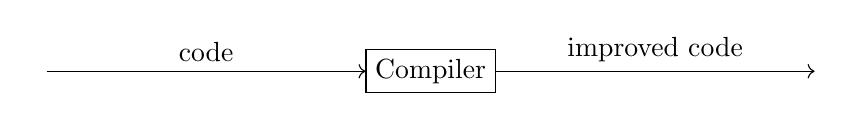
\begin{tikzpicture}
\node (a) at (-5,0) {};
\node (b) at (0,0) [shape=rectangle, draw] {Compiler};
\node (c) at (5,0) {};

\draw [->] (a) -- (b) node [midway, above] {code} ;
\draw [->] (b) -- (c) node [midway, above] {improved code} ;
%\draw [->] (b) -- (c) node [midway, above, text width=3cm, align=center] {improved\\code} ;
\end{tikzpicture}
 \caption[What is a Compiler]{A compiler is a program that takes code as input and outputs an improved version of that code.}
  \label{F.whatiscompiler}
\end{figure}
%----------------------------------------------------------

To illustrate the first principle, if you had a program that output the numbers from $1..10$ and the compiler transformed it so that it output one of e.e. cummings's poems, then clearly the compiler did not preserve the meaning of the original program.

The second principle is a bit less clear. If the code is a program, and you want to execute your program, then transforming your source code into an executable program would be an improvement. But suppose your source was a C program and the output was an equivalent Java program. Would that be an improvement?

This definition of a compiler is deliberately broad. The preprocessor for a C compiler (often a separate program from the C compiler) is considered a compiler. \LaTeX, which was used to typeset this book, is a compiler. Indeed, any converter program can be considered a compiler given this definition. For the sake of this book (and most compiler courses), we will primarily restrict ourselves to compilers where the input is a programming language. The output, however, does not need to be executable code. It can be any form of ``improved'' code.

\chapter{Compiler Structure}
Compilers are typically broken into two broad pieces: the front-end and the back-end. The frond-end deals with language specific issues. The back-end deals with target machine specifics.

A C compiler would need a very different front-end compared with a Haskell compiler because the syntax of the languages is very different. One way to view the front-end of the compiler is that it answers the question, ``Is this a valid program?'' If you feed a Scheme program into an R compiler, the answer would certainly by ``No''. If a Java program that was missing a semicolon was fed into a Java compiler, the answer would also be, ``No'', but for very different reasons.

The back-end of a compiler deals with target specific issues. The back-end for a compiler that targets the Java Virtual Machine (JVM) would be different than the back-end for a compiler that targets and ARM processor. Both of those would be different from a C preprocessor that simply outputs text.

Separating the front-end from the back-end makes sense because they are logically quite different, but it also makes sense because if they are properly designed, you can mix and match different front-ends and back-ends. Suppose you had a really good C compiler, but you wanted to port it to target a different machine. There would be no reason to rewrite the front-end. The C language is the same no matter what machine you are targeting. So if you wrote a new back-end and attached it to your existing front-end, you would now have a new compiler. Mixing can go the other way as well. Starting with the same really good C compiler, suppose you wanted a compiler for a different language (such as Go). There is no reason to rewrite the back-end, simply create a front-end for the new language and attach it to your existing back-end, and you have a new compiler.

For this mixing and matching to work seamlessly, there needs to be a common interface between the front-ends and the back-ends. This interface is typically called an Intermediate Representation (IR) --- see Chapter~\ref{chapter.IR}. The front-end translates the language into the IR, and the back-end translates the IR to the target representation. This is illustrated in Figure~\ref{figure.compiler_structure}

%----------------------------------------------------------
\begin{figure}[hbt]
\centering
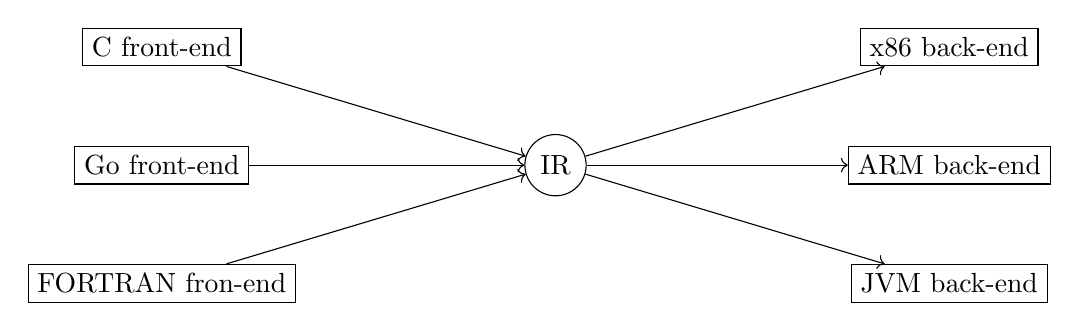
\begin{tikzpicture}
\node (a) at (-5,1.5) [shape=rectangle, draw]{C front-end};
\node (b) at (-5,0) [shape=rectangle, draw] {Go front-end};
\node (c) at (-5,-1.5) [shape=rectangle, draw]{FORTRAN fron-end};
\node (d) at (0,0)  [shape=circle, draw]{IR};
\node (e) at (5,1.5) [shape=rectangle, draw]{x86 back-end};
\node (f) at (5,0) [shape=rectangle, draw] {ARM back-end};
\node (g) at (5,-1.5) [shape=rectangle, draw]{JVM back-end};

\draw [->] (a) -- (d)  ;
\draw [->] (b) -- (d)  ;
\draw [->] (c) -- (d)  ;
\draw [->] (d) -- (e)  ;
\draw [->] (d) -- (f)  ;
\draw [->] (d) -- (g)  ;
\end{tikzpicture}
 \caption[Compiler Structure]{A properly structured compiler allows you to have multiple language-specific front-ends joined to multiple target-specific back-ends. The two a joined using an intermediate representation.}
  \label{figure.compiler_structure}
\end{figure}
%----------------------------------------------------------

Compiler front-ends typically contain two components: A scanner (aka tokenizer or lexer), and a parser. Scanners are discussed in detail in Part~\ref{part.scanner} and parsers are discussed in Part~\ref{part.parser}.

Most computer program source code comes in the form of a stream of characters (a text file). The scanner turns the stream of characters into a stream of tokens. For example, it the scanner read the characters ``\code{some_variable_name}'', it would output the single token \code{IDENTIFIER}. For a longer example, the string ``\code{int main() \{ printf("hello world"\\n); \}}'' would be converted to the tokens ``\code{TYPE IDENTIFIER ( ) \{ IDENTIFIER ( STRING_LIT ) ; \}}''.

Note: Programmers normally format their code to make it ``pretty''. The code in the above examples was not formatted to emphasize that to a compiler, code is just a stream of characters.

The parser takes a stream of tokens and decides whether that stream of tokens makes up a valid program (more specifically a ``compilation unit'') in the language. The parser only looks at the syntax of the language. As a result, ``valid program'' only means ``a program that is syntactically correct''. It does not mean ``a bug free program''.

\chapter{Intermediate Representations} \label{chapter.IR}

\part{Scanning} \label{part.scanner}

\chapter{Regular Expressions}

A scanner turns a stream of characters into a stream of tokens. To facilitate this conversion, most compilers make use of regular expressions to define tokens. Many programmers are familiar with regular expressions from non-compiler contexts. Examples include using an asterisk (*) as a wildcard in a file name, or specifying patterns for the \code{grep} utility. Different programs use different syntax for specifying regular expressions. In this section a minimalist syntax for all regular expressions is presented. Most programs that interpret regular expressions enhance this syntax in various ways to make writing regular expressions easier, but the added syntax does not add extra capabilities.

Regular expressions include the following features:
\begin{mydesc}[10em]
	\item[Concatenation] Concatenation is gluing two strings end-to-end. For example, concatenating ``\texttt{ab}'' with ``\texttt{bc}'' yields the string ``\texttt{abcd}''.
  \item[Alternation] Alternation means to choose exactly one from a set of alternatives. Regular expressions use the vertical bar (\texttt{|}) to mean alternation. So the expression \texttt{a | b | c} means to choose either an '\texttt{a}', a '\texttt{b}', or a '\texttt{c}'.
	\item[Grouping] Parenthesis can be used for grouping operations much as they can in algebraic expressions.
	\item[Kleene Closure] Kleene Closure means to take zero or more instances of a string. Kleene Closure is denoted by an asterisk (\texttt{*}). So, for example, \texttt{x*} means zero or more '\texttt{x}' characters. Kleene Closure has higher precedence that concatenation so that \texttt{ab*} means \texttt{a(b*)} not \texttt{(ab)*}.
\end{mydesc}

In addition to these operations, the $\Lambda$ symbol is used to represent an empty string (a string with no characters in it).

The most common enhancements to this syntax are as follows:
\begin{mydesc}
\item[zero or one] The question mark (\texttt{?}) indicates zero or one of an item so that \texttt{a?} means the same as \texttt{($\Lambda$ | a)}.
\item[one or more] The plus sign (\texttt{+}) is similar to Kleene Closure, but it is one-or-more not zero-or-more so that \texttt{a+} means the same as \texttt{aa*}.
\item[character range] Square brackets (\texttt{[]}) can be used to specify a character range so that \texttt{[a-m]} means any single character in the range '\texttt{a}' through '\texttt{m}'.
\end{mydesc}

If we want a regular expression for integer constants, we could try
\begin{quote}\texttt{[0-9]+}\end{quote}
but this allows any number of leading zeros. A better expression would be:
\begin{quote}\texttt{[1-9][0-9]*}\end{quote}
This fixes the leading zero problem, but it does not allow the number zero. This can be fixed as follows:
\begin{quote}\texttt{0 | ([1-9][0-9]*)}\end{quote}
If we want to allow negative numbers, we could add an optional minus sign:
\begin{quote}\texttt{0 | (-?[1-9][0-9]*)}\end{quote}

\textbf{Exercises}

\begin{enumerate}
\item Write a regular expression for a string containing any odd number of the letter \texttt{a}.
\item Write a regular expression for C (or Java) variable names. Valid characters include upper and lower case letters, digits, and the underscore (\texttt{\_}).
\item Write a regular expression for a string containing any number (including zero) of a positive even number of \texttt{a}'s followed by an add number of \texttt{b}'s. The following are valid strings: \texttt{aaaabbb}, \texttt{aabaabaabbb}, \texttt{aaaaaabbbbbaabaabaab}. The following are not valid strings: \texttt{aaab}, \texttt{aaaabbbaa}, \texttt{bbbaab}.
\item For the previous question, state why each of the non-valid strings are non-valid.
\item Write a regular expression for a floating-point constant. The following rules apply: 
\begin{enumerate}
\item The integer part cannot have leading zeros unless the integer part is zero. 
\item If there is a decimal point, it must be followed by at least one digit.
\item The decimal part must not have trailing zeros unless the decimal part is zero.
\end{enumerate}
\end{enumerate}

\chapter[Creating a Scanner]{Creating a Scanner from Regular Expressions}

To specify a scanner for a compiler, a developer could specify a regular expression for each token type. But how do you go from that specification to code that can actually process the input? This chapter discusses the algorithms used to convert regular expressions into a scanner. The general process is to convert the regular expression into a finite automaton. The finite automaton can then be evaluated using a simple table look-up on each character.

\section{Finite Automata}
Finite Automata (aka State Machines) consist of a finite number of states and transitions between states. One state is defined as the start state, and any number of states can be defined as final states. They are often drawn as diagrams as illustrated in Figure~\ref{F.FA_1}.

The start state in an FA is signified by an inbound arrow that doesn't originate from another state. Processing always starts in the start state. Final states are signified by a double circle. Transitions are labeled by the letter that is used to move from one state to another. 

%----------------------------------------------------------
\begin{figure}[hbt]
\centering
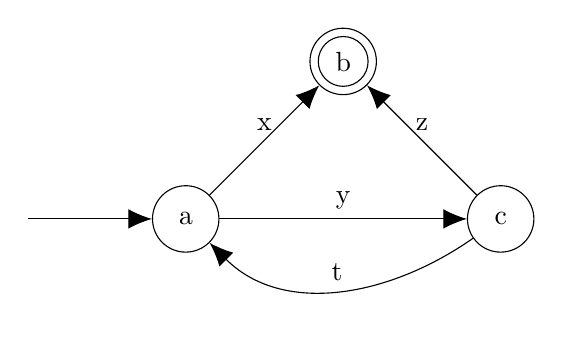
\begin{tikzpicture}

\fastart {-4, -2};
\fanonterminalnode {-2,-2}{a};
\faterminalnode {0,0}{b};
\fanonterminalnode {2,-2}{c};

\fatransition{start}{a}{};
\fatransition{a}{b}{x};
\fatransition{a}{c}{y};
\fatransition{c}{b}{z};
\faarctransition {c}{a}{t}{215}{315};

\end{tikzpicture}
 \caption[Sample Finite Automaton]{This is a sample FA. Node $a$ is the start state (it has an incoming arrow from nowhere). State $b$ is a final state (signified by the double-circle). The transitions are labeled by what letter is used to move from one state to another.}
  \label{F.FA_1}
\end{figure}
%----------------------------------------------------------

Using the FA in Figure~\ref{F.FA_1}, and the input $ytx$, the processing starts in State~$a$ (the start state). The $y$ is used to transition to State~$c$. The $t$ is used to transition back to State~$a$. The $x$ is used to transition to State~$b$. Since the input is exhausted while in a final state, the string is accepted by the FA.

Two conditions can cause a string to be rejected: 
\begin{enumerate}
\item If the input is exhausted and the current state isn't a final state. The input $yty$ illustrates this case.
\item If there is no outbound transition on the current letter. The input $yx$ illustrates this case.
\end{enumerate}

Given these rules for processing FA's, it should be clear that the FA in Figure~\ref{F.FA_1} is equivalent to the regular expression \texttt{(yt)* (x | yz)}

\subsection{Non-deterministic Finite Automata}

The FA illustrated in Figure~\ref{F.FA_1} is a Deterministic Finite Automaton (DFA). It is deterministic in the sense that for each character that is processed, the FA has exactly one choice on what to do. There is another class of FA's known as Non-deterministic Finite Automata (NFA's). With NFA's, for a given input, there is the potential for multiple choices on what to do. The choices can take two forms:
\begin{enumerate}
\item Multiple outbound edges labeled with the same letter. If that letter is read, any of the outbound edges labeled with that letter can be taken. This is illustrated by the edges from Node~$a$ labeled $z$ in Figure~\ref{F.FA_2}.
\item Edges labeled $\Lambda$. These edges can be taken without consuming an input character. Node~$a$ has a $\Lambda$ transition meaning you can leave Node~$a$ without consuming any characters.
\end{enumerate}

%----------------------------------------------------------
\begin{figure}[hbt]
\centering
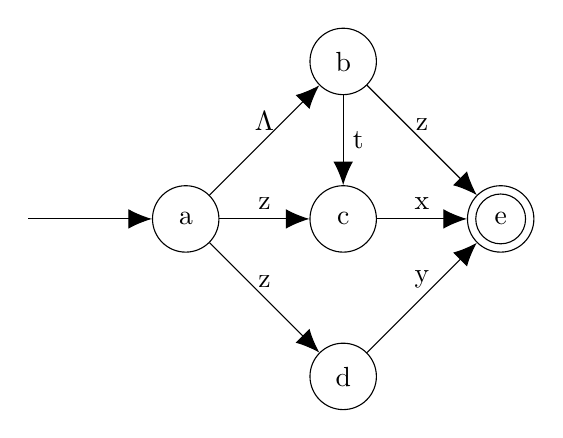
\begin{tikzpicture}

\fastart {-4, 0};
\fanonterminalnode {-2,0}{a};
\fanonterminalnode {0,2} {b};
\fanonterminalnode {0,0} {c};
\fanonterminalnode {0,-2} {d};
\faterminalnode {2,0} {e};

\fatransition{start}{a}{};
\fatransition{a}{b}{$\Lambda$};
\fatransition{a}{c}{z};
\fatransition{a}{d}{z};
\fatransition{b}{e}{z};
\farighttransition{b}{c}{t};
\fatransition{c}{e}{x};
\fatransition{d}{e}{y};

\end{tikzpicture}
 \caption[Sample Non-deterministic Finite Automaton]{This is a sample NFA. Node $a$ has multiple outbound transitions on $z$. It also has an outbound transition on $\Lambda$ meaning you could leave Node~$a$ without consuming any characters.}
  \label{F.FA_2}
\end{figure}
%----------------------------------------------------------

The NFA in Figure~\ref{F.FA_2} accepts the following stings:
\begin{mydesc}[2em]
	\item[$z$] This string is accepted by following the $\Lambda$ transition to Node~$b$ and then using the $z$ to transition to Node~$e$.
	\item[$tx$] This string is accepted by following the $\Lambda$ transition to Node~$b$ and then using the $t$ to transition to Node~$c$ and the $x$ to transition to Node~$e$.
	\item[$zx$] This string is accepted by using the $z$ to transition to Node~$c$ and then using the $x$ to transition to Node~$e$.
	\item[$zy$] This string is accepted by using the $z$ to transition to Node~$d$ and then using the $y$ to transition to Node~$e$.
\end{mydesc}

NFA's aren't any more powerful than DFA's--anything you can do with an NFA you can also do with a DFA\footnote{Section~Figure~\ref{S.Subset.Construction} gives a construction that can turn any NFA into an equivalent DFA. This is sufficient to argue that anything that can be done with an NFA can also be done with a DFA.}. The reason for introducing NFA's is that converting from a regular expression to code that accepts strings matching that regular expression makes use of NFA's.

\section{Thompson's}

The first step in converting a regular expression to executable code is to convert it to an equivalent NFA. For this conversion, we are going to use Thompson's Construction\footnote{Credited to Ken Thompson, the originator of the Unix operating system.}. The beauty of Thompson's construction is that it is a mechanical process -- one that doesn't require any creative thought. In other words, it can be automated. A computer program can be written to perform this conversion.

%----------------------------------------------------------
\begin{figure}[htb]
\centering

%\scalebox{.7}{
\begin{subfigure}[b]{0.45\textwidth}
\centering
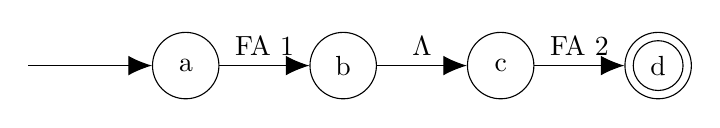
\begin{tikzpicture}
\fastart {0, 0};
\fanonterminalnode {2,0} {a};
\fanonterminalnode {4,0} {b};
\fanonterminalnode {6,0} {c};
\faterminalnode {8,0} {d};

\fatransition{start}{a}{};
\fatransition{a}{b}{FA 1};
\fatransition{b}{c}{$\Lambda$};
\fatransition{c}{d}{FA 2};

%\node at (5,-1) {Concatenation};
%\node at (5,-2) {};
\end{tikzpicture}
\caption{Concatenation}\label{F.Thompsons.Concatenation}
\end{subfigure}
%}

%\scalebox{.7}{
\begin{subfigure}[b]{0.45\textwidth}
\centering
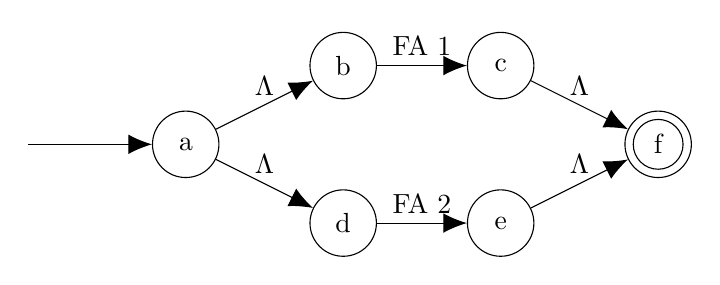
\begin{tikzpicture}
\fastart {0, 0};
\fanonterminalnode {2,0} {a};
\fanonterminalnode {4,1} {b};
\fanonterminalnode {6,1} {c};
\fanonterminalnode {4,-1} {d};
\fanonterminalnode {6,-1} {e};
\faterminalnode {8,0} {f};

\fatransition{start}{a}{};
\fatransition{a}{b}{$\Lambda$};
\fatransition{b}{c}{FA 1};
\fatransition{c}{f}{$\Lambda$};

\fatransition{a}{d}{$\Lambda$};
\fatransition{d}{e}{FA 2};
\fatransition{e}{f}{$\Lambda$};
%\node at (5,-2) {Alternation};
%\node at (5,-3) {};
\end{tikzpicture}
%}
\caption{Alternation}\label{F.Thompsons.Alternation}
\end{subfigure}

%\scalebox{.7}{
\begin{subfigure}[b]{0.45\textwidth}
\centering
%Kleene Closure
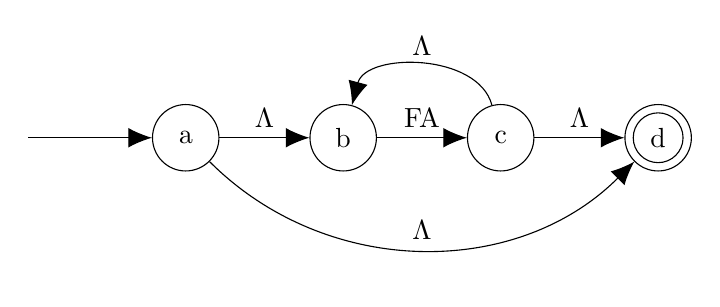
\begin{tikzpicture}
\fastart {0, 0};
\fanonterminalnode {2,0} {a};
\fanonterminalnode {4,0} {b};
\fanonterminalnode {6,0} {c};
\faterminalnode {8,0} {d};

\fatransition{start}{a}{};
\fatransition{a}{b}{$\Lambda$};
\fatransition{b}{c}{FA};
\fatransition{c}{d}{$\Lambda$};
\faarctransition {a}{d}{$\Lambda$}{315}{225};
\faarctransition {c}{b}{$\Lambda$}{105}{75};

%\node at (5,-2) {Kleene Closure};
%\node at (5,-3) {};
\end{tikzpicture}
%}
\caption{Kleene Closure}\label{F.Thompsons.KleeneClosure}
\end{subfigure}

 \caption[Thompson's Construction]{Thompson's Construction method makes use of these three diagrams. For each diagram, the FA(s) being composed are represented as two nodes (the start and end nodes) labeled $FA$, $FA 1$, or $FA 2$.}
  \label{F.Thompsons}
\end{figure}
%----------------------------------------------------------

If two FA's each have a single start state and a single final state, and if the start state doesn't have any inbound edges and the final state doesn't have any outbound edges, then the two FA's can be composed by connecting the end state of one FA to the start state of the other using a $\Lambda$ transition. Thompson's Construction makes use of this fact by creating composed FA's for each operation supported by regular expressions (concatenation, alternation, and Kleene Closure). An NFA can be built for any regular expression simply by composing it one small piece at a time using Thompson's three diagrams. Figure~\ref{F.Thompsons} shows the three base diagrams.

The trick to using Thompson's construction is to NOT be creative. Each FA built with Thompson's has a single start and a single final state. The diagram can be dropped as-is directly into the next step in the construction. Nodes never need to be erased, and each composition should be drawn exactly as shown in Figure~\ref{F.Thompsons}.

Let's illustrate by doing several constructions. First, let's construct an NFA for \texttt{a (b | c)}. It's best to start with the inner most operation (in this case \texttt{(b | c)}) and work out. So first draw the alternation diagram as shown below:

\begin{center}
\scalebox{.7}{
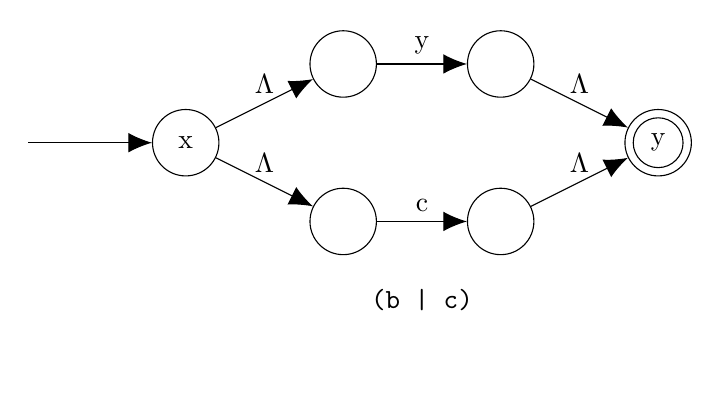
\begin{tikzpicture}
\fastart {0, 0};
\fanonterminalnode {2,0} {x};
\fanolabel {4,1} {b1};
\fanolabel {6,1} {b2};
\fanolabel {4,-1} {c1};
\fanolabel {6,-1} {c2};
\faterminalnode {8,0} {y};

\fatransition{start}{x}{};
\fatransition{x}{b1}{$\Lambda$};
\fatransition{b1}{b2}{y};
\fatransition{b2}{y}{$\Lambda$};

\fatransition{x}{c1}{$\Lambda$};
\fatransition{c1}{c2}{c};
\fatransition{c2}{y}{$\Lambda$};

\node at (5,-2) {\texttt{(b | c)}};
\node at (5,-3) {};
\end{tikzpicture}
} % end scaled box
\end{center}
The resulting diagram gets dropped into the \code{FA 2} position of the concatenation diagram as illustrated below. Note how the node labeled $x$ in the above diagram is in the location of the node labeled $c$ in the concatenation diagram, and the $y$ node is in the $d$ position.

\begin{center}
\scalebox{.7}{
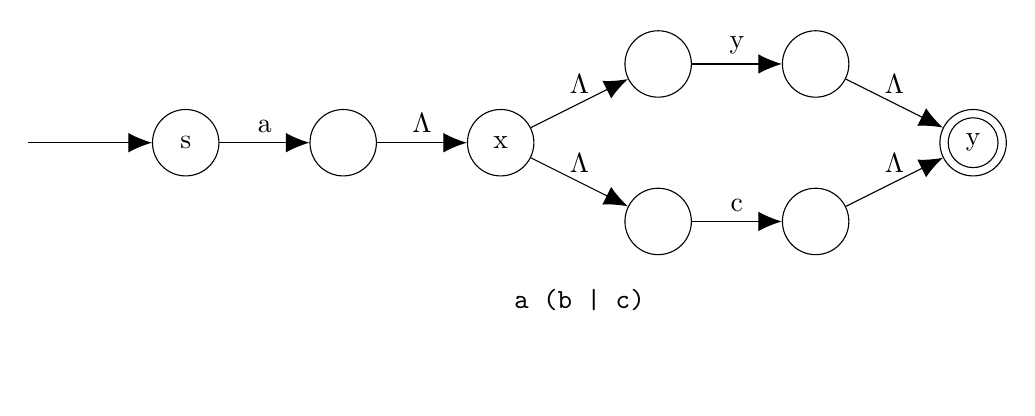
\begin{tikzpicture}
\fastart {0, 0};
\fanonterminalnode {2,0} {s};
\fanolabel {4,0} {a1};

\fanonterminalnode {6,0} {x};
\fanolabel {8,1} {b1};
\fanolabel {10,1} {b2};
\fanolabel {8,-1} {c1};
\fanolabel {10,-1} {c2};
\faterminalnode {12,0} {y};

\fatransition{start}{s}{};
\fatransition{s}{a1}{a};
\fatransition{a1}{x}{$\Lambda$};


\fatransition{x}{b1}{$\Lambda$};
\fatransition{b1}{b2}{y};
\fatransition{b2}{y}{$\Lambda$};

\fatransition{x}{c1}{$\Lambda$};
\fatransition{c1}{c2}{c};
\fatransition{c2}{y}{$\Lambda$};

\node at (7,-2) {\texttt{a (b | c)}};
\node at (7,-3) {};
\end{tikzpicture}
} % end scalebox
\end{center}

As a second example, let's construct an NFA for \texttt{a (b | c)*}. This is the same as the previous example, except that the alternation is wrapped in Kleene Closure. The alternation is, again, the innermost operation, and it is the same as in the previous example:

\begin{center}
\scalebox{.7}{
\begin{tikzpicture}
\fastart {0, 0};
\fanonterminalnode {2,0} {x};
\fanolabel {4,1} {b1};
\fanolabel {6,1} {b2};
\fanolabel {4,-1} {c1};
\fanolabel {6,-1} {c2};
\faterminalnode {8,0} {y};

\fatransition{start}{x}{};
\fatransition{x}{b1}{$\Lambda$};
\fatransition{b1}{b2}{y};
\fatransition{b2}{y}{$\Lambda$};

\fatransition{a}{c1}{$\Lambda$};
\fatransition{c1}{c2}{c};
\fatransition{c2}{y}{$\Lambda$};

\node at (5,-2) {\texttt{(b | c)}};
%\node at (5,-3) {};
\end{tikzpicture}
} % end scaled box
\end{center}

This is now dropped into the Kleene Closure construction:

\begin{center}
\scalebox{.7}{
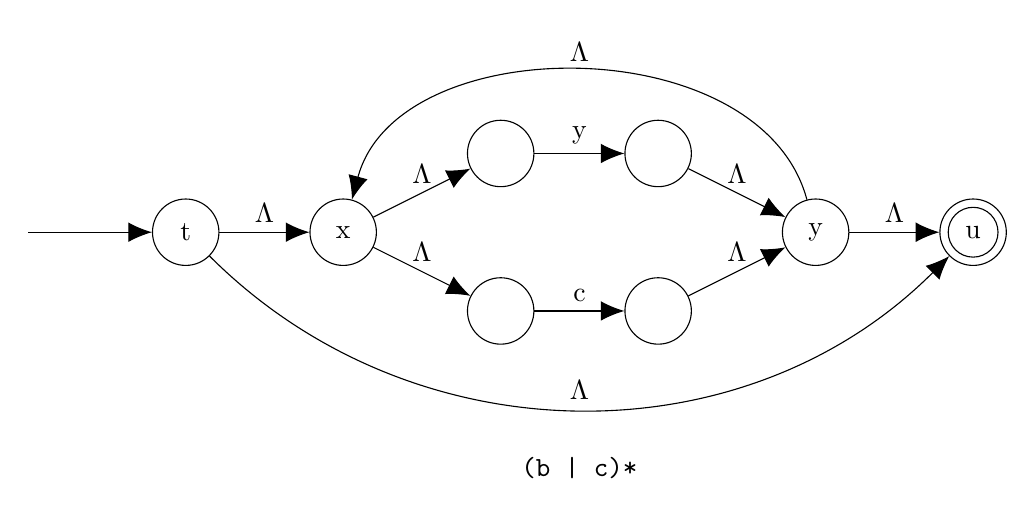
\begin{tikzpicture}
\fastart {0, 0};
\fanonterminalnode {2,0} {t}
\fanonterminalnode {4,0} {x};
\fanolabel {6,1} {b1};
\fanolabel {8,1} {b2};
\fanolabel {6,-1} {c1};
\fanolabel {8,-1} {c2};
\fanonterminalnode {10,0} {y};
\faterminalnode {12,0} {u};

\fatransition{start}{t}{};
\fatransition{t}{x}{$\Lambda$};
\fatransition{x}{b1}{$\Lambda$};
\fatransition{b1}{b2}{y};
\fatransition{b2}{y}{$\Lambda$};

\fatransition{x}{c1}{$\Lambda$};
\fatransition{c1}{c2}{c};
\fatransition{c2}{y}{$\Lambda$};

\fatransition{y}{u}{$\Lambda$};

\faarctransition {t}{u}{$\Lambda$}{315}{225};
\faarctransition {y}{x}{$\Lambda$}{105}{75};

\node at (7,-3) {\texttt{(b | c)*}};
\end{tikzpicture}
} % end scaled box
\end{center}

Finally, we drop this into the concatenation construction:
\begin{center}
\scalebox{.7}{
\begin{tikzpicture}
\fastart {0, 0};
\fanonterminalnode {2,0} {a}
\fanonterminalnode {4,0} {t}
\fanonterminalnode {6,0} {x};
\fanolabel {8,1} {b1};
\fanolabel {10,1} {b2};
\fanolabel {8,-1} {c1};
\fanolabel {10,-1} {c2};
\fanonterminalnode {12,0} {y};
\faterminalnode {14,0} {u};

\fatransition{start}{s}{};
\fatransition{s}{t}{$\Lambda$};
\fatransition{t}{x}{$\Lambda$};
\fatransition{x}{b1}{$\Lambda$};
\fatransition{b1}{b2}{y};
\fatransition{b2}{y}{$\Lambda$};

\fatransition{x}{c1}{$\Lambda$};
\fatransition{c1}{c2}{c};
\fatransition{c2}{y}{$\Lambda$};

\fatransition{y}{u}{$\Lambda$};

\faarctransition {t}{u}{$\Lambda$}{315}{225};
\faarctransition {y}{x}{$\Lambda$}{105}{75};

\node at (8,-3) {\texttt{a (b | c)*}};
\end{tikzpicture}
} % end scaled box
\end{center}

As a third example, \texttt{a* (b | c)}, includes a concatenation of two complex item (\texttt{a*} and \texttt{(b | c)} ). To construct this, first construct \texttt{a*}, then construct \texttt{(b | c)} and then use the concatenation construction to combine them. Here are the results:

\begin{center}
\scalebox{.7}{
\begin{tikzpicture}
\fastart {0, 0};
\fanonterminalnode {2,0} {t};
\fanolabel {4,0} {b};
\fanolabel {6,0} {c};
\fanonterminalnode {8,0} {u};

\fatransition{start}{t}{};
\fatransition{t}{b}{$\Lambda$};
\fatransition{b}{c}{a};
\fatransition{c}{u}{$\Lambda$};
\faarctransition {a}{u}{$\Lambda$}{315}{225};
\faarctransition {c}{b}{$\Lambda$}{105}{75};

\fanonterminalnode {10,0} {x};
\fanolabel {12,1} {b1};
\fanolabel {14,1} {b2};
\fanolabel {12,-1} {c1};
\fanolabel {14,-1} {c2};
\faterminalnode {16,0} {y};

\fatransition{u}{x}{$\Lambda$};
\fatransition{x}{b1}{$\Lambda$};
\fatransition{b1}{b2}{y};
\fatransition{b2}{y}{$\Lambda$};

\fatransition{x}{c1}{$\Lambda$};
\fatransition{c1}{c2}{c};
\fatransition{c2}{y}{$\Lambda$};

\node at (8,-2) {\texttt{a* (b | c)}};
%\node at (5,-3) {};
\end{tikzpicture}
} % end scaled box
\end{center}

It should be clear that Thompson's construction creates lots of $\Lambda$ transitions. This begs the question, ``isn't there an simpler way to draw these?''. The answer is in two parts. If by ``simpler'' you mean ``easier construction'', my answer would be ``no''. The whole point of Thompson's construction is that it is a simple mechanical process. It requires no creative thought. But if by ``simpler'' you mean a less complex result (one without all the $\Lambda$s), then the answer is ``yes''. The next section gives an algorithm to convert these complex NFAs into DFAs (diagrams without any $\Lambda$ transitions. The goal is not to make the diagram simpler, the goal is to get a DFA because they are easier to process in code.

\section{Subset Construction}\label{S.Subset.Construction}

To illustrate how an NFA could be processed, let's consider again the NFA for \texttt{a* (b | c)} presented in the last section, but presented again in Figure~\ref{F.subsetNFA}. In this figure, each node is labeled so they can be explicitly referred to. For each state, we can ask the question, ``What states could I wind up in if I encounter a particular letter in the input?''. For example, suppose we haven't consumed any input yet, what states could we be in? Clearly we could be in State~$1$, the start state, but because of the $\Lambda$ transitions, we could also be in states $2, 4, 5, 6, 8$. This set of states ($=\{1, 2, 4, 5, 6, 8\}$)\footnote{When specifying sets of characters,  it is often easier to read the list of items if each item is separated with a comma. This works unless the set included a comma (as sets of characters for a compiler often do). I will generally included commas for readability unless the set of characters includes punctuation (commas or other punctuation marks). I hope this will improve readability.}
forms a meta-state (let's call it $A$). From the meta-state~$A$, where could we wind up if we read an $a$. Since the meta-state~$A$ includes state~$2$, we can follow the $a$ to state~$3$. From there we can follow $\Lambda$s to $2, 4, 5, 6, 8$. This gives another meta-state. Let's call it $B = \{2, 3, 4, 5, 6, 8\}$. 

\begin{figure}[hbt]
\centering
\scalebox{.7}{
\begin{tikzpicture}
\fastart {0, 0};
\fanonterminalnode {2,0} {1};
\fanonterminalnode {4,0} {2};
\fanonterminalnode {6,0} {3};
\fanonterminalnode {8,0} {4};

\fatransition{start}{1}{};
\fatransition{1}{2}{$\Lambda$};
\fatransition{2}{3}{a};
\fatransition{3}{4}{$\Lambda$};
\faarctransition {a}{4}{$\Lambda$}{315}{225};
\faarctransition {3}{2}{$\Lambda$}{105}{75};

\fanonterminalnode {10,0} {5};
\fanonterminalnode {12,1} {6};
\fanonterminalnode {14,1} {7};
\fanonterminalnode {12,-1} {8};
\fanonterminalnode {14,-1} {9};
\faterminalnode {16,0} {10};

\fatransition{4}{5}{$\Lambda$};
\fatransition{5}{6}{$\Lambda$};
\fatransition{6}{7}{b};
\fatransition{7}{10}{$\Lambda$};

\fatransition{5}{8}{$\Lambda$};
\fatransition{8}{9}{c};
\fatransition{9}{10}{$\Lambda$};

\end{tikzpicture}
} % end scaled box
\caption[NFA produced by Thompson's]{This is the NFA produced by Thompson's for the regular expression \texttt{a* (b | c)}}
  \label{F.subsetNFA}
\end{figure}

We could continue to find new meta-states by enumerating all possible outbound inputs from each meta-state and then following the $\Lambda$s from the resulting states. The results are presented in Table~\ref{T.subsetTable1}.

\begin{table}[hbt]
\center
\begin{tabular}{l|l|l|l}
\hline
\textbf{meta-state} & \textbf{NFA states} & \textbf{input} & \textbf{resulting states} \\
\hline
A & 1, 2, 4, 5, 6, 8 & a & 2, 4, 5, 6, 8 \\
A & 1, 2, 4, 5, 6, 8 & b & 7, 10 \\
A & 1, 2, 4, 5, 6, 8 & c & 9, 10 \\
B & 2, 4, 5, 6, 8 & a & 2, 4, 5, 6, 8 \\
B & 2, 4, 5, 6, 8 & b & 7, 10 \\
B & 2, 4, 5, 6, 8 & c & 9, 10 \\
C & 7, 10 & a & - \\
C & 7, 10 & b & - \\
C & 7, 10 & c & - \\
D & 9, 10 & a & - \\
D & 9, 10 & b & - \\
D & 9, 10 & c & - \\
\hline
\end{tabular}
\caption[Result of subset construction]{The results of performing the subset construction on the NFA in Figure~\ref{F.subsetNFA}. An input of ``-'' means there are no valid inputs starting from this state. Resulting states of ``-'' mean there are no valid destinations from this state.}
\label{T.subsetTable1}
\end{table}

We need a formal algorithm for producing these tables. The steps are as follows:
\begin{enumerate}
\item From the start state, follow all $\Lambda$s. Follow as many as you can, not just one. This is known as the $\Lambda$ closure of a state: all states reachable from a given state following only $\Lambda$s. This set of states is labeled $A$ in the table.
\item Make multiple rows, one for each character in the source-language, for each meta-state not already in the table. Initially this is only meta-state~$A$, and for the example NFA in Figure~\ref{F.subsetNFA}, the characters in the source language are $a, b, c$ meaning three rows for each meta-state.
\item For each NFA state in the meta-state, if there is an outbound transition on the input, write down the destination state in the resulting states column.
\item Extend the list of states in the resulting states column by forming the $\Lambda$ closure of each state already in the column.
\item If there are any new unique sets of states in the resulting states column, give them a unique label and return to Step~2.
\end{enumerate}
The process will stop once all existing rows are filled in and no new rows get generated.

Let's use these rules to derive a table for the NFA below. Note: this NFA was \textbf{not} generated with Thompson's.

\begin{center}
\scalebox{.7}{
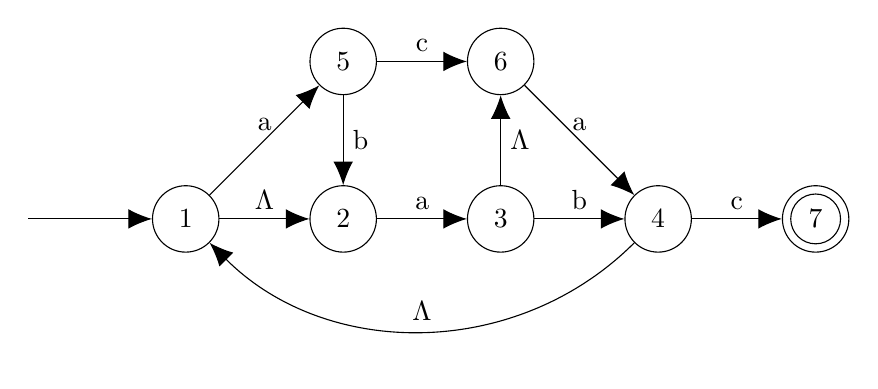
\begin{tikzpicture}
\fastart {0, 0};
\fanonterminalnode {2,0} {1};
\fanonterminalnode {4,0} {2};
\fanonterminalnode {6,0} {3};
\fanonterminalnode {8,0} {4};
\fanonterminalnode {4,2} {5};
\fanonterminalnode {6,2} {6};
\faterminalnode {10,0} {7};

\fatransition{start}{1}{};
\fatransition{1}{2}{$\Lambda$};
\fatransition{2}{3}{a};
\fatransition{3}{4}{b};
\farighttransition{3}{6}{$\Lambda$};
\fatransition{4}{7}{c};
\fatransition{1}{5}{a};
\fatransition{5}{6}{c};
\farighttransition{5}{2}{b};
\fatransition{6}{4}{a};
\faarctransition {4}{1}{$\Lambda$}{225}{315};

\end{tikzpicture}
} % end scaled box
\end{center}

Step~1 yields states 1 and 2, so this set becomes meta-state-$A$. There are three letters in the source language (a, b, c), so this yields the following rows:

\begin{center}
\small
\begin{tabular}{l|l|l|l}
\hline
\textbf{meta-state} & \textbf{NFA states} & \textbf{input} & \textbf{resulting states} \\
\hline
A & 1, 2 & a &  \\
A & 1, 2 & b &  \\
A & 1, 2 & c &  \\
\hline
\end{tabular}
\end{center}

Completing the first row, we can follow an $a$ from state 1 to 5, and from state 2 to 3. Add these two states to the resulting states column, and then follow the $\Lambda$s adding state 6. Label the set \texttt{ \{3, 5, 6\}} as meta-state~$B$ and add rows to the table:

\begin{center}
\small
\begin{tabular}{c|l|l|l|l}
\hline
& \textbf{meta-state} & \textbf{NFA states} & \textbf{input} & \textbf{resulting states} \\
\hline
1 & A & 1, 2 & a & B = 3, 5, 6 \\
2 & A & 1, 2 & b &  \\
3 & A & 1, 2 & c &  \\
4 & B & 3, 5, 6 & a &  \\
5 & B & 3, 5, 6 & b &  \\
6 & B & 3, 5, 6 & c &  \\

\hline
\end{tabular}
\end{center}

Completing rows 2 and 3, there are no $b$ nor $c$ transitions out of any of the states in meta-state~$A$, so the resulting states for both of these rows are empty.

Moving on to row 4, we can follow an $a$ from state 6 to state 4. We can then follow $\Lambda$s from 4 to 1 and 1 to 2 yielding meta-state $C$ containing states 1, 2, 4.

\begin{center}
\small
\begin{tabular}{c|l|l|l|l}
\hline
& \textbf{meta-state} & \textbf{NFA states} & \textbf{input} & \textbf{resulting states} \\
\hline
1 & A & 1, 2 & a & B = 3, 5, 6 \\
2 & A & 1, 2 & b & - \\
3 & A & 1, 2 & c & - \\
4 & B & 3, 5, 6 & a & C = 1, 2, 4 \\
5 & B & 3, 5, 6 & b & \\
6 & B & 3, 5, 6 & c & \\
7 & C & 1, 2, 4 & a & \\
8 & C & 1, 2, 4 & b & \\
9 & C & 1, 2, 4 & c & \\
\hline
\end{tabular}
\end{center}

For row 5, we can follow a $b$ from 3 to 4 and from 5 to 2. There are no $\Lambda$s from either 2 or 4, so meta-state~$D$ contains 2 and 4.

For row 6, we can follow a $c$ from 5 to 6. There are no $\Lambda$s from 6, so meta-state~$E$ contains only 6. Adding these new rows to the table, we have:

\begin{center}
\small
\begin{tabular}{c|l|l|l|l}
\hline
& \textbf{meta-state} & \textbf{NFA states} & \textbf{input} & \textbf{resulting states} \\
\hline
1 & A & 1, 2 & a & B = 3, 5, 6 \\
2 & A & 1, 2 & b & - \\
3 & A & 1, 2 & c & - \\
4 & B & 3, 5, 6 & a & C = 1, 2, 4 \\
5 & B & 3, 5, 6 & b & D = 2, 4 \\
6 & B & 3, 5, 6 & c & E = 6 \\
7 & C & 1, 2, 4 & a & \\
8 & C & 1, 2, 4 & b & \\
9 & C & 1, 2, 4 & c & \\
10 & D & 2, 4 & a & \\
11 & D & 2, 4 & b & \\
12 & D & 2, 4 & c & \\
13 & E & 6 & a & \\
14 & E & 6 & b & \\
15 & E & 6 & c & \\
\hline
\end{tabular}
\end{center}

Completing row 10, we can follow an $a$ from 1 to 5 and 2 to 3. The $\Lambda$ closure adds 6. This set of states is already labeled $B$, so we don't need to add any rows to the table.

For Row 11, there are no outbound edges on $b$ so the resulting states is empty.

For Row 12, we can follow a $c$ from 4 to 7. This new meta-state is labeled $F$.

\begin{center}
\small
\begin{tabular}{c|l|l|l|l}
\hline
& \textbf{meta-state} & \textbf{NFA states} & \textbf{input} & \textbf{resulting states} \\
\hline
1 & A & 1, 2 & a & B = 3, 5, 6 \\
2 & A & 1, 2 & b & - \\
3 & A & 1, 2 & c & - \\
4 & B & 3, 5, 6 & a & C = 1, 2, 4 \\
5 & B & 3, 5, 6 & b & D = 2, 4 \\
6 & B & 3, 5, 6 & c & E = 6 \\
7 & C & 1, 2, 4 & a & B\\
8 & C & 1, 2, 4 & b & -\\
9 & C & 1, 2, 4 & c & F = 7 \\
10 & D & 2, 4 & a & \\
11 & D & 2, 4 & b & \\
12 & D & 2, 4 & c & \\
13 & E & 6 & a & \\
14 & E & 6 & b & \\
15 & E & 6 & c & \\
16 & F & 7 & a & \\
17 & F & 7 & b & \\
18 & F & 7 & c & \\
\hline
\end{tabular}
\end{center}

For row 10, we can follow the a from 2 to 3 and then the $\Lambda$ to 6. This is meta-state~$G$.

For row 11, there are no outbound transitions on $b$, so the resulting states is empty.

For row 12, we can follow a $c$ from 4 to 7. This is already labeled $F$.

\begin{center}
\small
\begin{tabular}{c|l|l|l|l}
\hline
& \textbf{meta-state} & \textbf{NFA states} & \textbf{input} & \textbf{resulting states} \\
\hline
1 & A & 1, 2 & a & B = 3, 5, 6 \\
2 & A & 1, 2 & b & - \\
3 & A & 1, 2 & c & - \\
4 & B & 3, 5, 6 & a & C = 1, 2, 4 \\
5 & B & 3, 5, 6 & b & D = 2, 4 \\
6 & B & 3, 5, 6 & c & E = 6 \\
7 & C & 1, 2, 4 & a & B\\
8 & C & 1, 2, 4 & b & -\\
9 & C & 1, 2, 4 & c & F = 7 \\
10 & D & 2, 4 & a & G = 3, 6\\
11 & D & 2, 4 & b & - \\
12 & D & 2, 4 & c & F \\
13 & E & 6 & a & \\
14 & E & 6 & b & \\
15 & E & 6 & c & \\
16 & F & 7 & a & \\
17 & F & 7 & b & \\
18 & F & 7 & c & \\
19 & G & 3, 6 & a & \\
20 & G & 3, 6 & b & \\
21 & G & 3, 6 & c & \\
\hline
\end{tabular}
\end{center}

For Row 13, we can follow an $a$ from 6 to 4 and then $\Lambda$s to 1 and 2. This is already labeled $C$.

For Rows 13-18, there are no available outbound transitions, so the resulting states are empty.

The transitions for Row 19 are the same as for Row 13, so the result is $C$.

For Row 20, we can follow a $b$ from 3 to 4 and then $\Lambda$s give us meta-state $C$.

For Row 21, there are no outbound transitions on $c$ so the resulting state is empty.

This gives us the following table:

\begin{center}
\small
\begin{tabular}{c|l|l|l|l}
\hline
& \textbf{meta-state} & \textbf{NFA states} & \textbf{input} & \textbf{resulting states} \\
\hline
1 & A & 1, 2 & a & B = 3, 5, 6 \\
2 & A & 1, 2 & b & - \\
3 & A & 1, 2 & c & - \\
4 & B & 3, 5, 6 & a & C = 1, 2, 4 \\
5 & B & 3, 5, 6 & b & D = 2, 4 \\
6 & B & 3, 5, 6 & c & E = 6 \\
7 & C & 1, 2, 4 & a & B\\
8 & C & 1, 2, 4 & b & -\\
9 & C & 1, 2, 4 & c & F = 7 \\
10 & D & 2, 4 & a & G = 3, 6\\
11 & D & 2, 4 & b & - \\
12 & D & 2, 4 & c & F \\
13 & E & 6 & a & C\\
14 & E & 6 & b & - \\
15 & E & 6 & c & - \\
16 & F & 7 & a & - \\
17 & F & 7 & b & - \\
18 & F & 7 & c & - \\
19 & G & 3, 6 & a & C \\
20 & G & 3, 6 & b & C\\
21 & G & 3, 6 & c & - \\
\hline
\end{tabular}
\end{center}

All rows are filled in, so we are done.

\textbf{Important note:} The procedure is to follow the input out of the NFA states and then follow the $\Lambda$s. A common mistake is to follow the $\Lambda$s out of the NFA states. For example, when filling out the last row, even though there is a $\Lambda$ from state 3, we don't follow it because we are only looking for transitions on $c$.

The subset construction was supposed to turn an NFA into a DFA, but it appears to have just produced a table. We can take the information in our final table from the example we just completed and summarize it in Figure~\ref{F.transitionTable}.

%----------------------------------------------------------
\begin{figure}[hbt]
\centering

\small
\begin{tabular}{l|l|l}
\hline
\textbf{From} & \textbf{transition on} & \textbf{To} \\
\hline
A & a & B \\
B & a & C \\
B & b & D \\
B & c & E \\
C & a & B\\
C & c & F \\
D & a & G \\
D & c & F \\
E & a & C\\
G & a & C \\
G & b & C\\
\hline
\end{tabular}
\caption[Transition table for DFA]{A summary of the table derived in this section. Each row contains the start state, and input character, and the resulting state if that character is found while in the start state.}
  \label{F.transitionTable}
\end{figure}
%----------------------------------------------------------

This is known as a transition table. It is fairly straight forward to convert this table into a DFA (and a DFA into a transition table). Create states for each state in the table (the union of the From and To columns). The start state is always $A$, and any meta-state that included a final state in the original NFA is a final state in the DFA (in this case State~$F$). The resulting DFA is as follows:

\begin{center}
\scalebox{.7}{
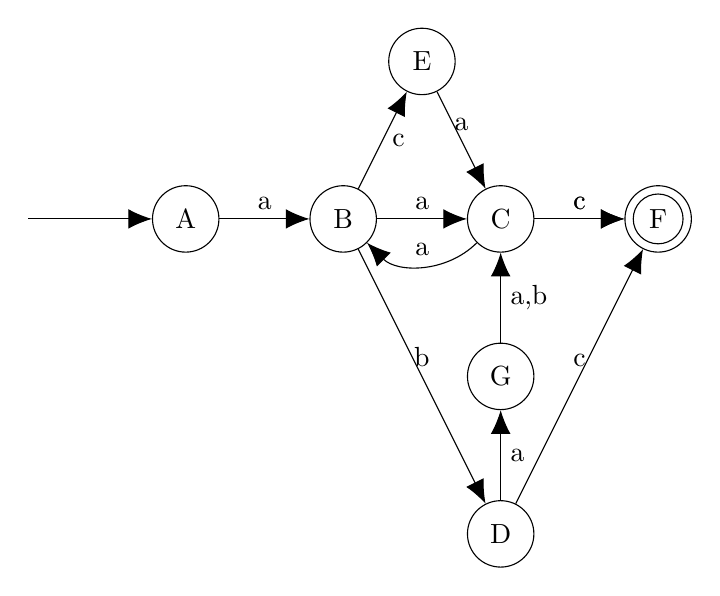
\begin{tikzpicture}
\fastart {0, 0};
\fanonterminalnode {2,0} {A};
\fanonterminalnode {4,0} {B};
\fanonterminalnode {6,0} {C};
\fanonterminalnode {6,-4} {D};
\fanonterminalnode {5,2} {E};
\faterminalnode    {8,0} {F};
\fanonterminalnode {6,-2} {G};

\fatransition{start}{A}{};
\fatransition{A}{B}{a};
\fatransition{B}{C}{a};
\fatransition{C}{F}{c};
\fatransition{C}{F}{c};
%\faarctransition{B}{D}{b}{270}{180};
\fatransition{B}{D}{b};
\farighttransition{D}{G}{a};
\farighttransition{G}{C}{a,b};
%\faarctransition{D}{F}{c}{0}{270};
\fatransition{D}{F}{c};
\farighttransition{B}{E}{c};
\fatransition{E}{C}{a};
\faarctransition {C}{B}{a}{225}{315};

\end{tikzpicture}
} % end scaled box
\end{center}

Does the subset construction always result in a DFA, or might it result in another NFA? The answer is that it always results in a DFA for the following two reasons:
\begin{enumerate}
\item The \emph{input} column never has $\Lambda$s, so the resulting FA will not have any $\Lambda$ transitions.
\item When generating rows, each meta-state has exactly one row for each input character. As a result, there will never be multiple outbound transitions for the same character.
\end{enumerate}
The consequence is that the resulting FA has no non-determinism and is therefore a DFA.

%%%%%%%%%%%%%%%%%%%%%%%%%%%%%%%%% Chapter %%%%%%%%%%%%%%%%%%%%%%%%%%%%%%%%%%
\chapter{Scanner Code}
The previous chapter presented algorithms for converting an arbitrary regular express into a transition table for a deterministic finite automata. The next question is, what do we do with that table? This chapter answers that question.

\section{Processing Transition Tables}\label{S.ScannerCode}
A DFA is a state diagram, and the transition table can be used as a lookup table for performing state transitions. Before showing the code for processing the lookup table, let's make one more modification to the table presented in Figure~\ref{F.transitionTable}. Instead of one row for each state-input combination, we will present the table as one row per state, and one column for each input possibility. Here is the result:

\begin{center}
\small
\begin{tabular}{l|c|c|c}
\hline
\textbf{State} & \textbf{a} & \textbf{b} & \textbf{c} \\
\hline
A & B & - & - \\
B & C & D & C \\
C & B & - & F \\
D & G & - & F \\
E & C & - & - \\
G & C & C & - \\
\hline
\end{tabular}
\end{center}

This table can be represented as a 2D array. The left-most column does not need to be stored as it simply gives the row index (converting from letters to suitable numbers). The current state is used as the row index and the just-read character is used as the column index. This results in the code in Listing~\ref{L.transitionTable}.

\begin{mylisting}
\centering
\begin{verbatim}
1  state = 0;
2  while (more_input_available)
3  {
4     input = next_character();
5  	 state = table[state][input];
6  }
7  if (state == final_state) 
8     return found;
9  else
10     return not_found;
\end{verbatim}
\caption{Pseudo-code for processing a transition table.}
\label{L.transitionTable}
\end{mylisting}

This code makes some problematic simplifying assumptions. First of all, how should the code deal with non-existent transitions (all the dashes in the table)? A simply solution is to add an error state to the table. All the dashes get changed to that error state, and all the columns for that error state return back to the same state: once you're in the error state, you're stuck there.

The second problem is that the table only has three columns one each for the three input characters. How do you convert from the character read (probably a number in ASCII or Unicode). There are several possible solutions. If the compiled language is defined over ASCII characters (particularly if it is 7-bit ASCII) then the table can be extended to have a row for each possible input character. 

With Unicode, this is less workable. For UTF-8 a similar scheme could be used, but the table would need additional rows to handle multi-byte characters. For UTF-16 or larger, the transition table would be so large, it would likely be unworkable. It would be possible to convert the UTF-16 to UTF-8 (they both encode the complete Unicode character set) and then use a 256 column wide table. This would cost the compiler time at the expense of a potentially smaller table.

Since this is A Very Simple compiler book, I will not delve into character conversions. Instead I'll assume the compiled language can use (or convert to) a reasonable sized character set.

\subsection{Replacing the table with code}

There are many space/speed trade-offs in computer algorithms (such as executing code to convert from UTF-16 to UTF-8 to have a narrower transition table). There are also trade-offs between code size and data size. The code presented in Listing~\ref{L.transitionTable} was very compact, but it required a potentially large data table. There is an alternative implementation that requires very little data, but a large amount of code. This is illustrated in Listing~\ref{L.switchStatement}.

\begin{mylisting}
\centering
\begin{verbatim}
1  state_0:
2  input = next_character();
3  switch (input)
4  {
5  	  case 'a': goto state_1;
6     case 'b': goto state_2;
7     case 'c': goto state_done;
8     default:  goto state_error;
9  }
10
11  state_1:
12  input = next_character();
13  switch (input)
14  {
15     case 'x': goto state_0;
16     case 'b': goto state_5;
17     case EOF: goto state_done;
18     default:  goto state_error;
19  }
    ...
\end{verbatim}
\caption{Alternative pseudo-code for processing a transition table. This just a sample to illustrate the form of the code. The actual \code{switch} statements would be determined based on the transition table.}
\label{L.switchStatement}
\end{mylisting}

This version of the code uses \code{switch} statements to move from state to state. Essentially, each row of the transition table is encoded into a \code{switch} statement. \code{goto} statements\footnote{Normally, \code{goto} statements are considered an unforgivable evil in code. This is one of the few instances were they are useful, and not evil} are used to jump to the block of code that handles the new state.

One advantage of this implementation is that the code (and data) is not affected by large character sets. Each \code{switch} statement only has branches for characters that matter. Any unused characters in the character set will not appear in the code. The flip side of this is that if there are states that can handle a large number of characters (for example, the regular expression for an identifier in a UNICODE language could include any of a very large number of characters) would require a large number of \code{case} branches.

\subsection{Performance considerations}\label{S.scannerperformance}
So, which of these two implementations is better. The short answer is: that depends.

The first consideration is how efficiently the implementation language implements a \code{switch} statement. If the \code{switch} statements are translated to an equivalent \code{if elsif else} statement, then there is likely little advantage to the \code{switch} form of implementation. For the following discussion, we'll assume an efficient \code{switch} implementation.

\subsubsection{Implementation size}\label{S.scannersize}
If we consider the memory size required by the implementation, the following observations can be made:
\begin{enumerate}
\item The code for the transition table version is quite small. The size of the code does not change with the complexity of the language being scanned: the same code can process any transition table.
\item The data table for the transition table version can be quite large. Its size depends on the number of characters in the character set for the language being compiled, and on the number of states that are required to implement the scanner.
\item The code for the \code{switch} implementation can be very large. It depends on the number of states that are required to implement the scanner and also on the number of valid characters in each state.
\item The data required for the \code{switch} implementation is small: a single integer to store the current character.
\end{enumerate}

If the transition table is sparse (few valid characters in each row), then the \code{switch} implementation may require less memory because the \code{switch} statements only include code for the necessary characters whereas the transition table version must store the entire table--even the cells for transitions that are invalid. However, if the table is dense (many valid characters in each (or many) rows, then the transition table version is likely to require less memory. Each valid entry in the table requires more code in the \code{switch} version, however the table size doesn't change with density in the transition table implementation.

\subsubsection{Locality of Reference}\label{S.scannerlocality}

\needswork{}


\section{Processing multiple regular expressions}\label{S.MultiScanner}
Algorithm for multiple RE's
\needswork{}
\chapter{Automatically Generated Scanners}
here is a description of flex.
\needswork{}

\part{Parsing} \label{part.parser}
The scanner converts the input stream from a stream of characters into a stream of tokens. The parser tries to make sense of the stream of tokens. In particular, it answers the question, ``Does this sequence of tokens for a valid program?''

\chapter{Context Free Grammars}
Regular expressions are used to define the tokens a compiler processes. We also need a mechanism to define the syntax of the language a compiler processes. Context Free Grammars are used for this purpose.

A Context Free Grammar (CFG) is made up a a list of productions of the form:

\indent this symbol can be replaced by this collection of symbols

A production in a CFG consists of a left hand side and a right hand side. The left hand side gives the symbol that can be replaced. The right hand side gives the list of symbols that can replace the symbol on the left. The two sides are typically separated 
either by an arrow ( $\rightarrow$ ) 
or sometimes a colon-colon-equals ( ::= ). 
A sample production that indicates that the symbol \code{A} 
can be replaced by \code{X Y Z} is given below:

\cfg{A}{X Y Z}

Symbols in CFGs are of two flavors: non-terminals are those that appear on the left hand side of a production. They are non-terminals because they can be replaced by other symbols. Terminals are those symbols that never appear on the left hand side. They are ``terminal'' because they can never be replaced. For ease of reading, non-terminals are usually given in UPPERCASE. terminals are given in lowercase. CFGs also need a start symbol - the symbol that is the starting point for derivations. The start symbol is often either \code{S} or \code{START}, but if neither is specified, the left hand side of the first production is considered the start symbol.

Here is a more complete CFG example. The productions have been numbered for easy reference.

\begin{enumerate}
\item \cfg{S}{a S b}
\item \cfg{S}{$\lambda$}
\end{enumerate}

There are only two productions. The first one says that the start symbol (\code{S}) can be replaced with \code{a S b}. Note that this is a recursive rule because the \code{S} appears on both sides. The second production says that \code{S} can be replaced with nothing.

What can we do with this CFG? Let's do some derivations. Starting with the start symbol and Production 1, we can get the string \code{a S b}. If we then use Production 2, we are left with the string \code{a b}. Since there are no more non-terminals, we are done.

What if we invoked Production 1 more than once? The first invocation produces \code{a S b}. The next invocation produces \code{aa S bb}. Each invocation adds another \code{a} and \code{b}. When we finally invoke Production 2, we are left with a string of \code{a}'s followed by the same number of \code{b}'s.

zzz
\chapter {Top-down recursive-descent parsers}
\needswork{}

\chapter {Bottom-up parsers}
\needswork{}

\chapter {Automatically generated parsers}
Description of bison.
\needswork{}

\part {Semantic Processing}
\needswork{}

\chapter {Syntax vs. Semantics}
\needswork{}

\chapter {Type systems}
\needswork{}

\chapter {Implementation details}
\needswork{}

\part{The Back-end}
\needswork{}

\chapter {The Visitor Pattern}
\needswork{}

\chapter {Code generation}
\needswork{}

\chapter {Optimization}
\needswork{}

\part {\LaTeX sample code}

\begin{description}
\item[Description List] Each description list item has a term followed by the
description of that term.

\item[Bunyip] Mythical beast of Australian Aboriginal legends.
\end{description}

\section{Theorem-Like Environments}

The following theorem-like environments (in alphabetical order) are available
in this style.

\begin{acknowledgement}
This is an acknowledgement
\end{acknowledgement}

\begin{algorithm}
This is an algorithm
\end{algorithm}

\begin{axiom}
This is an axiom
\end{axiom}

\begin{case}
This is a case
\end{case}

\begin{claim}
This is a claim
\end{claim}

\begin{conclusion}
This is a conclusion
\end{conclusion}

\begin{condition}
This is a condition
\end{condition}

\begin{conjecture}
This is a conjecture
\end{conjecture}

\begin{corollary}
This is a corollary
\end{corollary}

\begin{criterion}
This is a criterion
\end{criterion}

\begin{definition}
This is a definition
\end{definition}

\begin{example}
This is an example
\end{example}

\begin{exercise}
This is an exercise
\end{exercise}

\begin{lemma}
This is a lemma
\end{lemma}

\begin{proof}
This is the proof of the lemma.
\end{proof}

\begin{notation}
This is notation
\end{notation}

\begin{problem}
This is a problem
\end{problem}

\begin{proposition}
This is a proposition
\end{proposition}

\begin{remark}
This is a remark
\end{remark}

\begin{summary}
This is a summary
\end{summary}

\begin{theorem}
This is a theorem
\end{theorem}

\begin{proof}
[Proof of the Main Theorem]This is the proof.
\end{proof}

\appendix

\chapter{The First Appendix}

The \verb"\appendix" command should be used only once. Subsequent appendices can
be created using the Chapter command.

\chapter{The Second Appendix}

Some text for the second Appendix.

This text is a sample for a short bibliography. You can cite a book by making use of
the command \verb"\cite{KarelRektorys}": \cite{KarelRektorys}. Papers can be cited
similarly: \cite{Bertoti97}. If you want multiple citations to appear in a single set
of square brackets you must type all of the citation keys inside a single citation,
separating each with a comma. Here is an example: \cite{Bertoti97, Szeidl2001,
Carlson67}.

\begin{thebibliography}{9}
\bibitem {KarelRektorys}Rektorys, K., \textit{Variational methods in Mathematics,
Science and Engineering}, D. Reidel Publishing Company,
Dordrecht-Hollanf/Boston-U.S.A., 2th edition, 1975

\bibitem {Bertoti97} \textsc{Bert\'{o}ti, E.}:\ \textit{On mixed variational formulation
of linear elasticity using nonsymmetric stresses and displacements}, International
Journal for Numerical Methods in Engineering., \textbf{42}, (1997), 561-578.

\bibitem {Szeidl2001} \textsc{Szeidl, G.}:\ \textit{Boundary integral equations for
plane problems in terms of stress functions of order one}, Journal of Computational and
Applied Mechanics, \textbf{2}(2), (2001), 237-261.

\bibitem {Carlson67}  \textsc{Carlson D. E.}:\ \textit{On G\"{u}nther's stress functions
for couple stresses}, Quart. Appl. Math., \textbf{25}, (1967), 139-146.
\end{thebibliography}

\backmatter

\chapter{Afterword}

The back matter often includes one or more of an index, an afterword,
acknowledgments, a bibliography, a colophon, or any other similar item. In
the back matter, chapters do not produce a chapter number, but they are
entered in the table of contents. If you are not using anything in the back
matter, you can delete the back matter TeX field and everything that follows it.
\end{document}
